\documentclass[tikz]{standalone}
\usepackage{amsfonts}
\usepackage{amsmath}
\usepackage{amssymb}
\usepackage{tikz}
\begin{document}

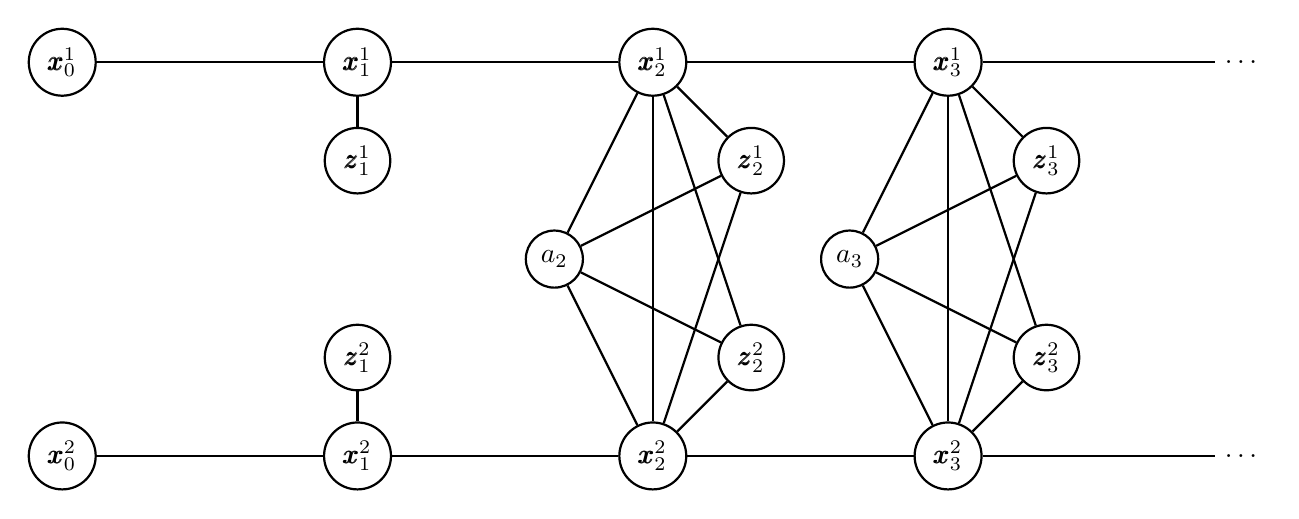
\begin{tikzpicture}

\begin{scope}[every node/.style={circle,thick,draw}]
	%Frame 1
	\node (x_0^1) at (-3.75, 0) {$\pmb{x}_{0}^{1}$};
	\node (x_0^2) at (-3.75, -5) {$\pmb{x}_{0}^{2}$};
	
	%Frame 2
	\node (x_1^1) at (0, 0) {$\pmb{x}_{1}^{1}$};
	\node (z_1^1) at (0, -1.25) {$\pmb{z}_{1}^{1}$};
	
	\node (z_1^2) at (0, -3.75) {$\pmb{z}_{1}^{2}$};
	\node (x_1^2) at (0, -5) {$\pmb{x}_{1}^{2}$};
	
	%Frame 3
	\node (x_2^1) at (3.75, 0) {$\pmb{x}_{2}^{1}$};
	
	\node (a_2) at (2.5, -2.5) {$a_{2}$};
	\node (z_2^1) at (5, -1.25) {$\pmb{z}_{2}^{1}$};
	\node (z_2^2) at (5, -3.75) {$\pmb{z}_{2}^{2}$};
	
	\node (x_2^2) at (3.75, -5) {$\pmb{x}_{2}^{2}$};
	
	%Frame 4
	\node (x_3^1) at (7.5, 0) {$\pmb{x}_{3}^{1}$};
	
	\node (a_3) at (6.25, -2.5) {$a_{3}$};
	\node (z_3^1) at (8.75, -1.25) {$\pmb{z}_{3}^{1}$};
	\node (z_3^2) at (8.75, -3.75) {$\pmb{z}_{3}^{2}$};
	
	\node (x_3^2) at (7.5, -5) {$\pmb{x}_{3}^{2}$};
\end{scope}

\begin{scope}[style={thick,draw}]
	%Frame 5
    \node (xdot1) at (11.25, 0) {\dots};
    \node (xdot2) at (11.25, -5) {\dots};
\end{scope}

\begin{scope}[style={thick,draw}]
	%Frame 1
	\path [-] (x_0^1) edge node {} (x_1^1);
	\path [-] (x_0^2) edge node {} (x_1^2);
	
	%Frame 2
	\path [-] (x_1^1) edge node {} (x_2^1);
	\path [-] (x_1^1) edge node {} (z_1^1);
	
	\path [-] (x_1^2) edge node {} (z_1^2);
	\path [-] (x_1^2) edge node {} (x_2^2);

	%Frame 3
	\path [-] (x_2^1) edge node {} (x_3^1);
	\path [-] (x_2^1) edge node {} (z_2^1);
	\path [-] (x_2^1) edge node {} (z_2^2);
	\path [-] (x_2^1) edge node {} (x_2^2);
	
	\path [-] (a_2) edge node {} (x_2^1);
	\path [-] (a_2) edge node {} (z_2^1);
	\path [-] (a_2) edge node {} (z_2^2);
	\path [-] (a_2) edge node {} (x_2^2);
	
	\path [-] (x_2^2) edge node {} (x_3^2);
	\path [-] (x_2^2) edge node {} (z_2^1);
	\path [-] (x_2^2) edge node {} (z_2^2);
		
	%Frame 4
	\path [-] (x_3^1) edge node {} (xdot1);
	\path [-] (x_3^1) edge node {} (z_3^1);
	\path [-] (x_3^1) edge node {} (z_3^2);
	\path [-] (x_3^1) edge node {} (x_3^2);
	
	\path [-] (a_3) edge node {} (x_3^1);
	\path [-] (a_3) edge node {} (z_3^1);
	\path [-] (a_3) edge node {} (z_3^2);
	\path [-] (a_3) edge node {} (x_3^2);
	
	\path [-] (x_3^2) edge node {} (z_3^1);
	\path [-] (x_3^2) edge node {} (z_3^2);
	\path [-] (x_3^2) edge node {} (xdot2);
\end{scope}

\end{tikzpicture}

\end{document}